\documentclass[11pt]{article}
\usepackage{UF_FRED_paper_style}
\usepackage{lipsum}
\usepackage{enumitem}
\usepackage{amsmath}
\usepackage{dsfont}
\usepackage{mathtools}
\usepackage{bm}
\usepackage{array}
\usepackage{color}
\usepackage{multicol}
\usepackage[labelfont=bf]{caption}
\usepackage{lstbayes} % Bayes version of listings package
\usepackage{xcolor}
\usepackage{pdfpages}
\usepackage{titletoc}
\usepackage[toc,page]{appendix}

% appendix
\renewcommand\appendixpagename{Appendix}
\renewcommand\appendixtocname{Appendix}

% Code chunk setup
\definecolor{commentcolor}{HTML}{8F8F8F}
\definecolor{codegray}{rgb}{0.5,0.5,0.5}
\definecolor{codepurple}{HTML}{FFA500}
\definecolor{backcolor}{HTML}{FFFFFF}
\definecolor{fctcolor}{HTML}{C28100}
\lstdefinestyle{mystyle}{
    backgroundcolor=\color{backcolor},   
    commentstyle=\color{commentcolor},
    keywordstyle=\color{fctcolor},
    numberstyle=\tiny\color{codegray},
    stringstyle=\color{codepurple},
    basicstyle=\ttfamily\footnotesize,
    breakatwhitespace=false,         
    breaklines=true,                 
    captionpos=b,                    
    keepspaces=true,                 
    numbers=left,                    
    numbersep=5pt,                  
    showspaces=false,                
    showstringspaces=false,
    showtabs=false,                  
    tabsize=2
}
\lstset{style=mystyle}

%\doublespacing
%\singlespacing
\onehalfspacing

% table settings
\newcolumntype{P}[1]{>{\centering\arraybackslash}p{#1}}
\abovedisplayskip=0pt
\belowdisplayskip=0pt

% possesive citation
\newcommand\possecite[1]{\citeauthor{#1}'s (\citeyear{#1})}

% captions and notes
\newcommand\fnote[1]{\captionsetup{font=footnotesize}\caption*{\textit{#1}}}
\newcommand\minp[1]{\begin{minipage}{0.8\textwidth} #1 \end{minipage}}

% colored comments
\newcommand{\colcom}[2][red]{
\textcolor{#1}{#2}
}

\setitemize{itemsep = -0.5em}
\setlength{\parindent}{0pt}
\setlength{\parskip}{0.5em}
\setlength{\droptitle}{-5em} %% Don't touch

\title{\large Final Paper \\ ~ \\
\LARGE  Government Stability and Female Representation:\\
A Bayesian Replication of Krauss \& Kröber (2020)\footnote[1]{The replication files for this paper are publicly available on GitHub under \url{github.com/pitrieger/BaysianStats_FinalProject}.}}

\author{Pit Rieger\\
    \href{mailto:prieger@ethz.ch}{\texttt{prieger@ethz.ch}}\\
    19-951-102}

\date{\today}


%%%%%%%%%%%%%%%%%%%%%%%%%%%%%%%%%%%%%%%%%%%%%%%%%%%%%%%%%%%%%%%%%%%%%%%%%%%%%%%%%%%


\begin{document}

\maketitle

\bigskip
\bigskip
\bigskip
\bigskip
\begin{center}
    $\Huge \bigcirc$
\end{center}
\bigskip
\bigskip
\bigskip
\bigskip

\begin{abstract}
{\noindent\itshape
\lipsum[1]
}
\end{abstract}

\bigskip
\bigskip
\bigskip
\bigskip

\newpage

%\setcounter{tocdepth}{2}
%\tableofcontents
%\clearpage

\section{Introduction \& Research Question}
Empirical analyses of cabinet stability and duration have a long tradition in the political science literature (for an overview, see XXX). \textcite{LupiaStrøm1995} even trace this literature back to early works by \textcite{Bryce1921} and \textcite{Lowell1896}. A recent paper by \textcite{KK20} addresses the research question \textit{whether cabinets with a higher share of women are more stable.} Their findings suggest that indeed the share of women is negatively associated with the risk of early termination. In this paper, I seek to address this question by replicating \possecite{KK20} findings in a Bayesian framework. More specifically, I rely on Bayesian survival regression models as well as a zero-inflated Poisson regression. 

Scholars have identified several factors that increase the risk of early cabinet terminations. \textcite{SchleiterMorganJones2009} differentiate between government-specific, parliament-specific, and political-system-specific attributes. Government-specific attributes include the minority status of the government and whether it is a single-party or coalition government \parencite{StromSwindle2002}. Parliament-specific attributes are the fragmentation and polarization of the party system \parencite{KingEtAl1990}. Finally, the political system matters for example by determining the duration of the constitutional inter-election period \parencite{StromSwindle2002}. Moreover, with regard to constitutional power, \textcite{SchleiterMorganJones2009} show that systems in which cabinets can dissolve themselves are at a higher risk of early termination (see also Strøm \& Swindle, \citeyear{StromSwindle2002}).

In essence, \textcite{KK20} start by arguing that generally conflict lies at the heart of the factors that are associated with government stability. They further stipulate that leadership style determines the response to situations of conflict \parencite{KK20}. In this regard, a broad literature has found that on average, women are more likely to compromise and collaborate to dissolve conflict than men \parencite[e.g.][]{KellermanRhode2017women}. Taken together, these arguments lead them to "hypothesise that the presence of a female prime minister and female ministers positively impacts cabinet stability" \parencite[4]{KK20}.


\section{Methods \& Data}
\subsection{Data}
I will rely entirely on the replication data from \textcite{KK20}, which is available online and mostly stems from the ERDDA \parencite{ERD2014}, which contains 676 governments in 27 European countries\footnote{Full list of countries: Austria, Belgium, Denmark, Finland, France, Germany, Greece, Iceland, Ireland, Italy, Luxembourg, Netherlands, Norway, Portugal, Spain, Sweden, Great Britain, Bulgaria, Czechia, Estonia, Hungary, Latvia, Lithuania, Poland, Romania, Slovakia, Slovenia.}. Therefore, this section merely describes their specification of the data. The main variable of interest $Y_i$, $i = 1, ..., n$, is a right-censored random variable, representing the number of days that a given government was in office. Censoring takes place because for some governments, we cannot observe when they would have collapsed because they survived until the next regular election date. However, we implicitly assume that all governments would fail eventually as time $t \to \infty$, such that $Y_i < \infty$. In the following, $F_i$ is an indicator of whether government $i$ failed before the next regulation and consequently $C_i = 1-F_i$ an indicator of whether observation $i$ is censored. 

With respect to the substantive research question, \possecite{KK20} derive several covariates from the literature. I mostly follow their specification of the regression equation with some differences, discussed below. Table \ref{tab:summarystat} provides summary statistics of the covariates. The main independent variable is the share of female ministers and the gender of the head of government. Due to the fact that \textcite{KK20} find that the latter doesn't matter much and that very few cabinets have a female head of government to begin with, I restrict my analysis to the share of female ministers in the cabinet (Model 2 in their paper). This variable is computed across all ministers in a given government, irrespective of the duration of their tenure in government. The finding and expectation of \textcite{KK20} is that a higher share is associated with higher government stability. Further covariates are the ideological divisiveness, the effective number of parliamentary parties (ENPP), the length of the constitutional inter-election period (CIEP), the minority status of the cabinet and the maximum possible duration of the cabinet at the time of its formation. The ideological divisiveness is calculated by the maximum pairwise absolute distance between the left-right positions of all coalition parties where the left-right positions were taken from the Comparative Manifesto Project \parencite{CMP2018}. In this regard, the expectation is that ideologically divided coalitions are less stable than single-party governments or coalitions between ideologically close parties. The ENPP is measured as defined by \textcite{LaaksoTaagepera1979} and was taken from ParlGov \parencite{parlgov}. Again, \textcite{KK20} expect and find that the ENPP is associated with low government stability, because there are more options for alternative coalitions as well as more complex coalition bargaining \parencite[c.f.][]{Saalfeld2008}. The CIEP is a measure of the constitutional inter-election period in years and stems from \textcite{MullerStrom2008}, \textcite{Krauss2018}, as well as \possecite{KK20} own coding. The minority status of a cabinet is a simple indicator variable and was taken from ParlGov \parencite{parlgov}. \textcite{KK20} find that minority governments are generally at much greater risk of a short duration. However, the authors fail to mention that this is likely the result of the fact that minority government are often regarded as a last-resort option, e.g. when other alternatives have collapsed. A different literature argues that minority governments are just as stable, if not more stable than other types of government [CITE Oli, etc.]. Finally, the maximum possible duration of the cabinet at the time of its formation is measured in days to control for governments that come into office when there isn't much time left before the next scheduled election. The underlying data stems from the ERDDA \parencite{ERD2014} and ParlGov \parencite{parlgov}. Obviously, these cabinets will be terminated sooner \parencite{KK20}. 

\begin{table}[!htbp] \centering 
  \caption{Summary of covariates} 
  \label{tab:summarystat} 
\begin{tabular}{@{\extracolsep{5pt}}lcccc} 
& \multicolumn{1}{c}{\textbf{Percentage}} & \multicolumn{1}{c}{\textbf{Mean}} & \multicolumn{1}{c}{\textbf{SD}} & \multicolumn{1}{c}{\textbf{Range}}
\\\hline 
\hline \\[-1.8ex]  
Share of Women in Cabinet & & 13.389 & 13.427 & 0 $-$ 55\\ 
Ideological Divisiveness & & 18.42 & 20.07 & 0 $-$ 121.87  \\ 
ENPP & & 4.04 & 1.42 & 2 - 10.8\\ 
Max. Poss. Duration (normalized) & & 0 & 1.000 & -2.595 $-$ 1.627 \\\hline 
Decade: 1950 & 11  & & & \\ 
Decade: 1960 & 9.8 & & &   \\ 
Decade: 1970 & 11.7 & & &   \\ 
Decade: 1980 & 12.6 & & &   \\ 
Decade: 1990 & 18.8 & & &   \\ 
Decade: 2000 & 18.5 & & &   \\ 
Decade: 2010 & 12.9 & & &   \\ 
CIEP: 4      & 74.6 & & & \\ 
CIEP: 5      & 24.7 & & &  \\ 
Minority     & 33.1 & & & \\ 
\hline \\[-1.8ex] 
\end{tabular} 
\end{table} 

In some cases, I deviate from \possecite{KK20} operationalization and specification. First, I additionally control for the decade in which the government was inaugurated. The reason for this is that recent governments clearly have higher shares of female ministers, so the decade has the potential to be a confounder. Second, I treat the CIEP as a categorical instead of a numerical variable. The variable essentially reduces to cases with 3, 4, or 5 year cases, rendering its treatment as a continuous variable questionable. Third, I normalize the maximum duration for computational reasons. Finally, I do not adopt the use of time-varying coefficients in the model. Further extensions of my model should look into implementing this feature for survival models in a Bayesian framework. 

\subsection{Models}
\subsubsection{Exponential Survival Model}
Survival models are still often associated with a frequentist approach. Certainly easy to use \texttt{R}-packages, such as \texttt{Survival} \parencite{Rsurvival2020} have played a role in their popularity. At the same time, \texttt{rstanarm} \parencite{rstanarm2020} has only recently extended its range to survival models in the development version\footnote{\url{https://github.com/stan-dev/rstanarm/tree/feature/survival} (retrieved on 11 May 2021)}. Instead of relying on this à-la-carte option, I wrote the \texttt{Stan} code myself. However, Eren M. Elçi's blog post\footnote{\url{https://ermeel86.github.io/case_studies/surv_stan_example.html} (retrieved on 11 May 2021)} on Bayesian survival models was incredibly helpful to vectorize the posterior draws using \texttt{Stan}'s convenient logarithmic complementary cumulative distribution function (\texttt{*\_lccdf}).

If it wasn't for the censoring, discussed above, survival models could simply be estimated with standard regression models, such as gamma or Weibull regression. Given that we know the time at which censoring occurs, one way to account for censoring is to integrate the censored observations out of the likelihood function. Thus, the likelihood for a censored observation $j$ is given by 

\begin{align*}
\mathcal{L}_j (\theta) &= \int_{y_j}^{\infty} p(u_j|\theta_j) du_j \\
&= 1-\mathbb{P}_\theta(Y_j \leq y_j),
\end{align*}

which is the complementary cumulative distribution function (ccdf).

Thus, the likelihood of all observations can be written as 

\begin{align*}
    \mathcal{L}_{1:n}(\theta) = \prod_{i = 1}^n \left\{C_j (1-\mathbb{P}_{\theta_i}(Y_i \leq y_i)) + (1-C_i) p(y_i|\theta)\right\}
\end{align*}

or more conveniently after arranging the data into censored and uncensored observations of length $n_1$ and $n_2 = n - n_1$ 

\begin{align}
    \mathcal{L}_{1:n}(\theta) &= \mathcal{L}_{1:n_1}(\theta) + \mathcal{L}_{(n_1 + 1):n}(\theta) \nonumber \\
    &= \prod_{i = 1}^{n_1} (1-\mathbb{P}_{\theta_i}(Y_i \leq y_i)) \prod_{i = n_1 + 1}^n p(y_i|\theta_i).
    \label{eq:likelihood}
\end{align}

As a distributional assumption, I assume that the failure times are exponentially distributed with density function (pdf)

\begin{equation*}
    p(y_i|\theta_i) = \theta_i \exp(-\theta_i y_i)
\end{equation*}

and cumulative distribution function (cdf) 

\begin{equation*}
    \mathbb{P}_{\theta_i}(Y_i \leq y_i) = 1 - \exp(-\theta_i y_i)
\end{equation*}

such that the ccdf is simply
    
\begin{equation*}
    1 - \mathbb{P}_{\theta_i}(Y_i \leq y_i) = \exp(-\theta_i y_i).
\end{equation*}
    
In all cases, the covariates are included in the rate (inverse scale) parameter $\theta_i \in \mathbb{R}^+$ which is defined as 

\begin{equation*}
    \bm{\theta} = \exp(\beta_0 + \bm{X}\bm{\beta}). 
\end{equation*}

\subsubsection{Weibull Survival Model}
Another alternative is to change the distributional assumption to a Weibull distribution. This relaxes the assumption of a constant hazard rate that is made by the exponential model discussed above. Instead, the Weibull model allows for hazards to increase or decrease over time. 

No changes are necessary with respect to the general approach of integrating over censored observations, so the likelihood in equation \ref{eq:likelihood} remains. However, $\theta_i$ needs to be redefined to accommodate the two parameters of the Weibull distribution. I thus redefine $\theta_i = (\alpha, \sigma_i)$, $\alpha, \sigma \in \mathbb{R}^+$. Further, the pdf of the Weibull distribution is given by 

\begin{equation*}
    p(y_i|\theta_i) = \frac{\alpha}{\sigma_i} \left(\frac{y_i}{\sigma_i}\right) \exp\left(-\left(\frac{y_i}{\sigma_i}\right)^{\alpha}\right)
\end{equation*}

its cdf by

\begin{equation*}
    \mathbb{P}_{\theta_i}(Y_i \leq y_i) = 1 - \exp\left(-\left(\frac{y_i}{\sigma_i}\right)^{\alpha}\right)
\end{equation*}

and so its ccdf is

\begin{equation*}
    1 - \mathbb{P}_{\theta_i}(Y_i \leq y_i) = \exp\left(-\left(\frac{y_i}{\sigma_i}\right)^{\alpha}\right).
\end{equation*}

I then 

\subsection{Prior Selection}
Both the exponential and the Weibull model require priors for the intercept $\beta_0$ and the coefficients of the covariates $\bm\beta$. Since these are simple regression coefficients, I use jointly independent normal priors for all parameters. Formally, 

\begin{align*}
    \beta_0 &\sim \mathcal{N}(0, 100) \\
    \bm{\beta} &\sim \mathcal{N}_{p}(0, 5^2I),
\end{align*}
where $\mathcal{N}_p$ is the multivariate normal distribution and $I$ a $p\times p$ identity matrix. Note that the prior is much less informative for the intercept compared to the covariates. 

Finally, 

\section{Analysis}
\subsection{Convergence}
Figure \ref{fig:exp_convergence} shows the trace plots of all four chains for the regression parameters in the exponential survival model. Clearly, the chains have mixed well, which is also indicated by the $\hat{R}$-statistic, which is $1.0$ for all parameters in the model (not included here). This suggests that the algorithm has converged and that we can trust the posterior estimates from the model for the remainder of this paper. An analogous figure for the Weibull model can be found in the appendix and was excluded from this main section because it similarly shows good convergence.

\begin{figure}[!ht]
    \centering
    \minp{\caption{Traces of the parameters in the Exponential survival model.} \label{fig:exp_convergence}}
    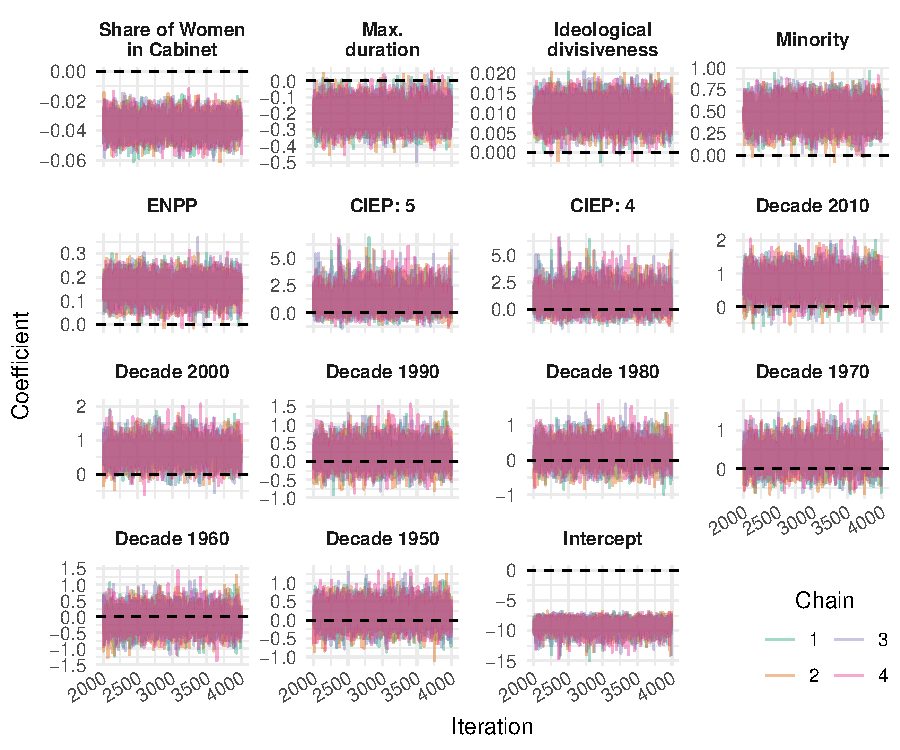
\includegraphics[width = 0.8\textwidth]{figures/fig2_exp_convergence.pdf}
\end{figure}

\subsection{Results}
Turning to the posteriors from the exponential model, Figure \ref{fig:exp_coefplot} shows that several covariates are clearly associated with a higher or lower government stability. Generally, negative effects are indicative of a higher government stability and positive effects of earlier termination. This can be verified by considering the expectation of our dependent exponential random variable $Y_i \sim \text{Expo}(\theta_i)$ which is given by $\mathbb{E}\left[Y_i\right] = 1/\theta_i$. Decreases in the linear predictor $\beta_0 + \bm{X_i\beta}$ thus lead to decreases in $\theta_i$ and finally an increase in  $\mathbb{E}\left[Y_i\right]$.

\begin{figure}[!ht]
    \centering
    \minp{\caption{Posterior densities of the coefficients in the exponential survival model.} \label{fig:exp_coefplot}}
    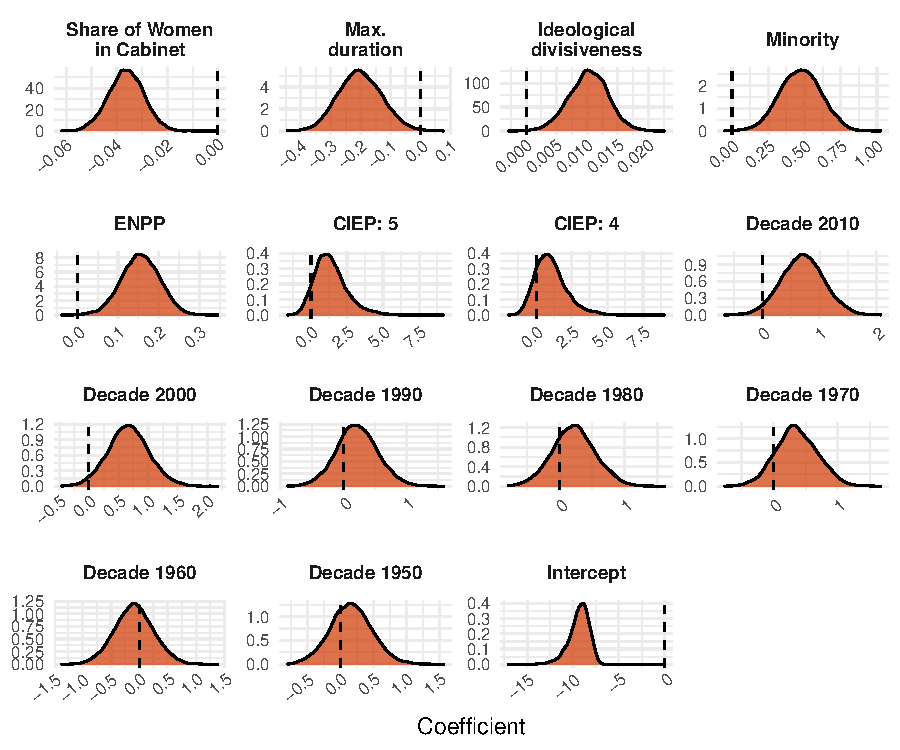
\includegraphics[width = 0.8\textwidth]{figures/fig1_exp_coefplot.pdf}
\end{figure}

The posteriors from the exponential model are in line with \possecite{KK20} finding that cabinets with higher shares of women also tend to last longer. Similarly, the longer the maximum possible duration at the time of government formation, the higher the stability of the government. In the opposite direction, minority governments, ideologically divided cabinets and cabinets arising from legislatures with a high effective number of parliamentray parties (ENPP) are clearly more likely to terminate sooner. With respect to the constitutional inter-election period (CIEP), the interpretation is more ambiguous. While longer CIEPs tend to be associated with lower stability, both densities cover the null comfortably. Finally, the results also show that recent cabinets, particularly in the 2000s and 2010s, tend to be less stable than cabinets in earlier decades. 

\begin{figure}[!ht]
    \centering
    \minp{\caption{Posterior predictive distribution for different shares of women in cabinet in the exponential survival model.} \label{fig:exp_posteriorpredict}}
    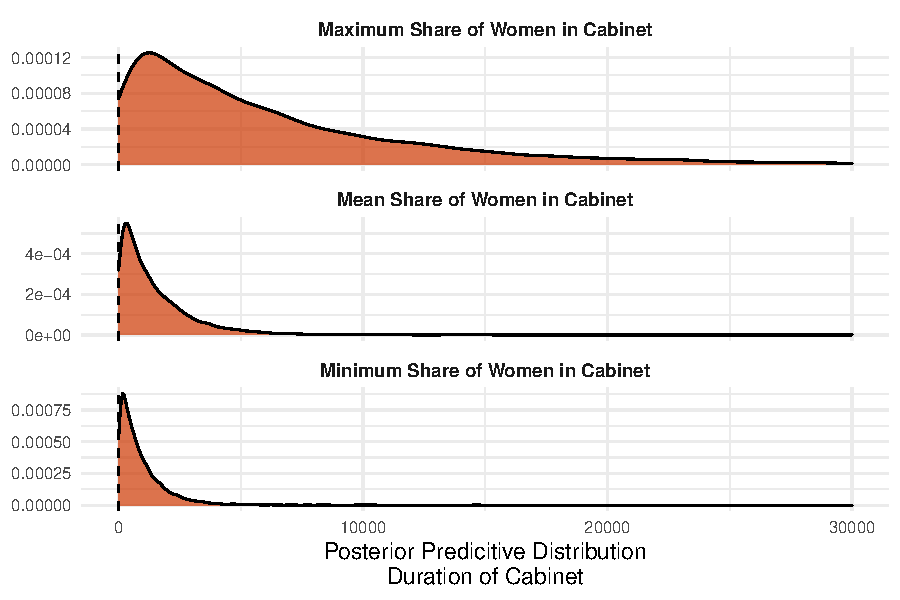
\includegraphics[width = 0.8\textwidth]{figures/fig3_exp_posteriorpredict.pdf}
\end{figure}

To further explore the main focus of \possecite{KK20} and this paper, Figure \ref{fig:exp_posteriorpredict} and \ref{fig:exp_survplot} visualize the magnitude of the effect of the share of women in cabinet. Figure \ref{fig:exp_posteriorpredict} depicts the posterior predictive distributions for different shares of women in the cabinet. The minimum, mean, and maximum reflect the sample values of female cabinet ministers and correspond to 0\%, 13.4\%, and 54.5\%, respectively. The remaining variables are set to encode a non-minority cabinet in the 2010's in a system with a CIEP of 4 years while holding all numeric variables constant at their respective sample mean. Clearly, the expected government duration increases substantively as a function of the share of women in cabinet. To illustrate, the median duration for the minimum, mean, and maximum share of women in cabinet is about 600, 990, and 4320 days, respectively. This can also be gathered from the survival functions for the same groups of cabinets, shown in Figure \ref{fig:exp_survplot}. For cabinets with high shares of women in the setting described above, the survival function is barely decreasing, indicating very high stability. For cabinets without any women on the other hand, the survival function decreases with less than 12.5\% of cabinets expected to survive at 2000 days, the empirical maximum duration (of course including right-censoring). 

\begin{figure}[!ht]
    \centering
    \minp{\caption{Survival function of the exponential survival model.} \label{fig:exp_survplot}}
    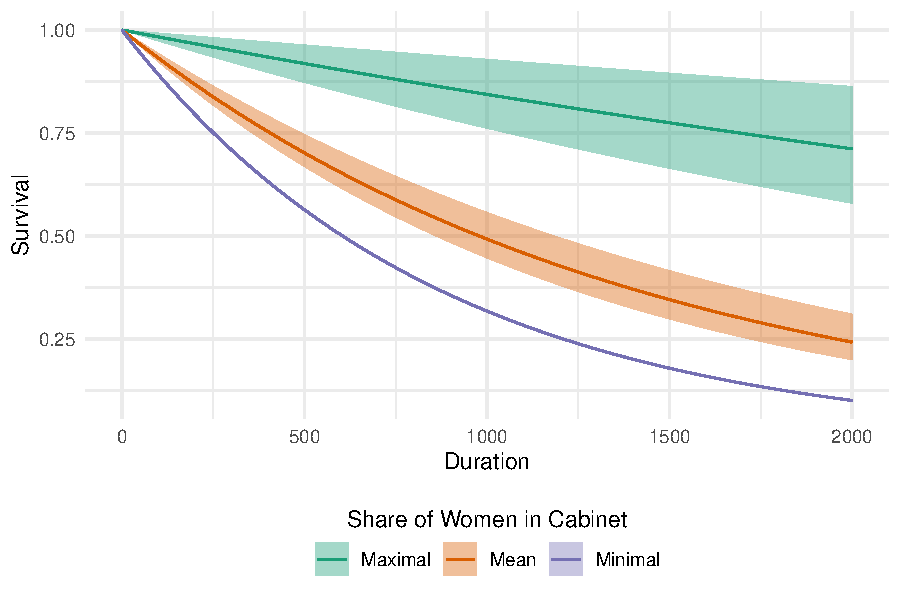
\includegraphics[width = 0.8\textwidth]{figures/fig4_exp_survplot.pdf}
    \minp{\fnote{\textbf{Note:} Shaded areas represent 95\% credible intervals, taking into account only the uncertainty in the coefficient for the share of women in cabinet. As a result, the purple line for the minimal share of women in cabinet doesn't have a shaded area, because that share is equal to zero, rendering the uncertainty zero as well. Instead, it be interpreted as a baseline survival function.}}
\end{figure}

However, the shape of the survival functions in Figure \ref{fig:exp_survplot} also reveals a weakness of assuming exponential survival times: The functional form of the exponential survival function, an implication of a constant hazard of termination, is theoretically questionable. Especially the steep initial decrease in the survival functions seems unrealistic. It seems more likely that cabinets what have a high probability of terminating very early are less likely to be formed in the first place. A survival function that reflects this would need to decrease slowly at first and then begin to decrease more at a later stage. Therefore, it is prudent to have a look at the more flexible Weibull distribution, which can accommodate such survival function shapes. Convergence diagnostics and a coefficient plot, analogous to Figures \ref{fig:exp_convergence} and \ref{fig:exp_coefplot}, can be found in the appendix, but were excluded from the main section because the results do not differ substantially from Figures \ref{fig:exp_convergence} and \ref{fig:exp_coefplot}. In fact, with respect to the coefficients of the covariates, the models are strikingly similar and no noteworthy inferential differences exist.

\begin{figure}[!ht]
    \centering
    \minp{\caption{Posterior predictive distribution for different shares of women in cabinet in the Weibull survival model.} \label{fig:weib_posteriorpredict}}
    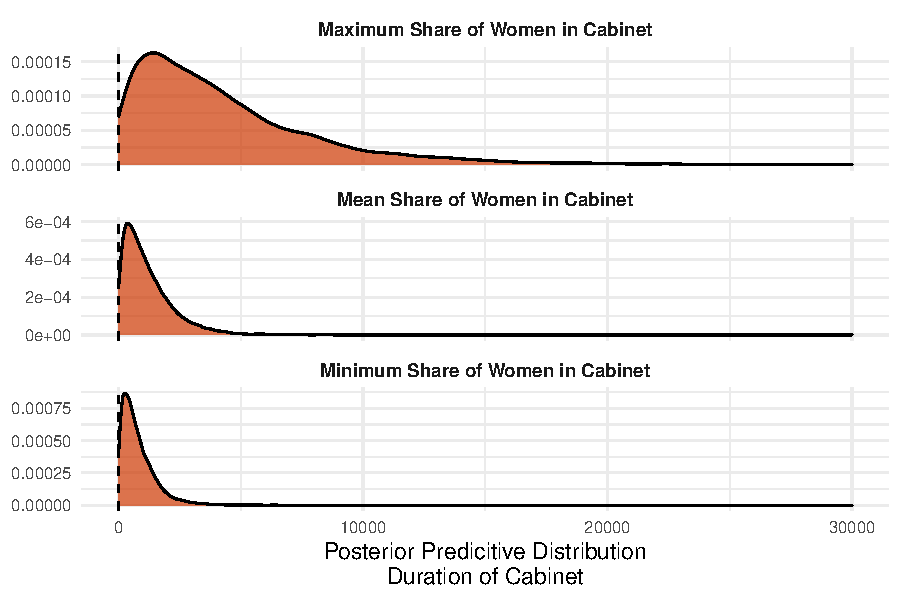
\includegraphics[width = 0.8\textwidth]{figures/fig3_weib_posteriorpredict.pdf}
\end{figure}

Finally, Figures \ref{fig:weib_posteriorpredict} and \ref{fig:weib_survplot} are analogous to Figures \ref{fig:exp_posteriorpredict} and \ref{fig:exp_survplot}, but were created from the Weibull model instead. They both indicate that there's some merit to the argument made above. The median duration for the minimum, mean, and maximum share of women in cabinet according to the posterior predictive distribution of the Weibull model, as shown in Figure \ref{fig:weib_posteriorpredict}, is about 610, 970, and 3330 days, respectively. Furthermore, the survival functions in Figure \ref{fig:weib_survplot} indeed don't decrease as steeply as in the exponential model. However, generally speaking, the difference between the Weibull model and the exponential model are rather minor. 

\begin{figure}[!ht]
    \centering
    \minp{\caption{Survival function of the Weibull survival model.} \label{fig:weib_survplot}}
    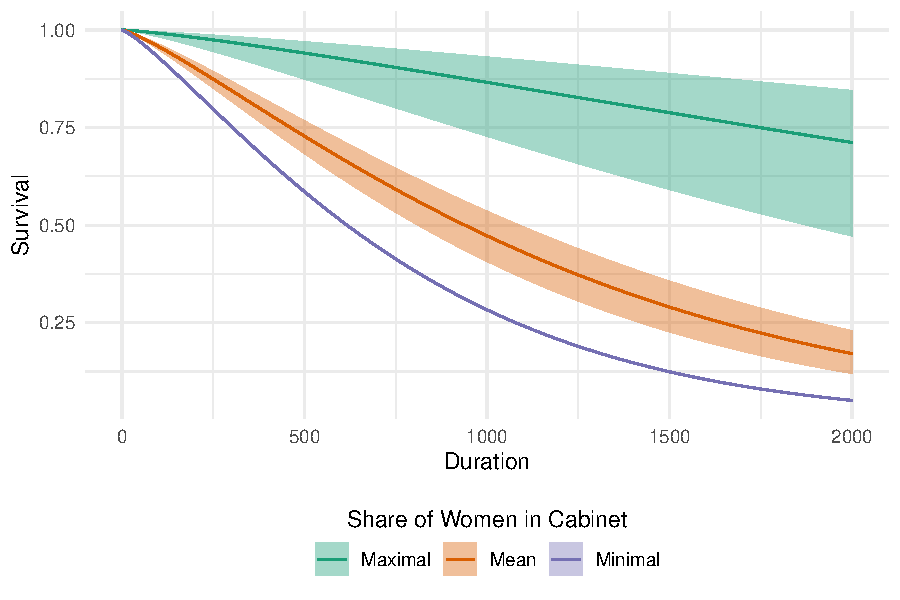
\includegraphics[width = 0.8\textwidth]{figures/fig4_weib_survplot.pdf}
\end{figure}

\subsection{Discussion}

\clearpage

\printbibliography

\newpage

\section{Appendix}

\setcounter{table}{0}
\renewcommand{\thetable}{A\arabic{table}}
\setcounter{figure}{0}
\renewcommand{\thefigure}{A\arabic{figure}}


\subsection{Stan Code}
\begin{lstlisting}[language=Stan, caption = {Stan Model Code}, captionpos = t, label = {code:stan}]
data {
    int<lower=0> n_event; // # uncensored obs         
    int<lower=0> n_censor; // # censored obs
    int<lower=0> p; // # covariates excluding intercept
    matrix[n_event,p] X_event; // uncensored obs design matrix 
    matrix[n_censor,p] X_censor; // censored  -----"----------
    vector<lower=0>[n_event] T_event; // uncensored survival times
    vector<lower=0>[n_censor] T_censor; // lower bound of censored
    survival times = censor time                  
}
parameters {
    real alpha;
    vector[p] beta;                                     
}
model {
    vector[n_event] lambda_event = exp(alpha + X_event * beta);
    vector[n_censor] lambda_censor = exp(alpha + X_censor * beta);
    alpha ~ normal(0, 100);
    beta ~ normal(0, 5);
    target += exponential_lpdf(T_event | lambda_event); 
    target += exponential_lccdf(T_censor | lambda_censor);  
}
\end{lstlisting}


\subsection{Zero-Inflated Poisson Regression}
Since the interest is more on the association between survival time and the share of female ministers in the cabinet, the problem can also be approached differently, i.e. outside the survival modelling framework. Typically it is roughly known when the next regular elections will be held. At the start of each government, we can thus already tell what the maximum number of possible days in office for that government will be. Denoting this maximum as $m_i$, we can compute the number of days that the government fell short of reaching that maximum as 

\begin{equation*}
    \widetilde{Y}_i = m_i - Y_i.
\end{equation*}

We thus have a count variable $\widetilde{Y}_i$ that can be modelled as a zero-inflated Poisson random variable. The likelihood of this model is therefore given by 
\begin{equation*}
    \mathcal{L}_i(\theta) = \begin{cases}
    \pi_i + (1-\pi_i) e^{-\lambda_i} \lambda_i^{0} & \text{, $\tilde{y}_i = 0$} \\
    (1-\pi_i) \frac{e^{-\lambda_i} \lambda_i^{y_i}}{\tilde{y}_i!} & \text{, otherwise}
    \end{cases}
\end{equation*}

where $\bm\theta = (\bm\pi, \bm\lambda)$ can be defined via logistic and log link functions, respectively, such that 

\begin{align*}
    \bm\pi &= (1 + \exp(-(\alpha + \bm{X} \bm\beta)))^{-1} \\
    \bm\lambda &= \exp(\nu+ \bm{Z} \bm\gamma)/ 
\end{align*}

\end{document}